\documentclass[tikz,border=5pt]{standalone}
\usepackage{fontspec}
\setmainfont{Times New Roman}
\usepackage{unicode-math}
\setmathfont{Cambria Math}
\usetikzlibrary{shapes.geometric,positioning,fit,backgrounds,arrows.meta,calc}

\begin{document}
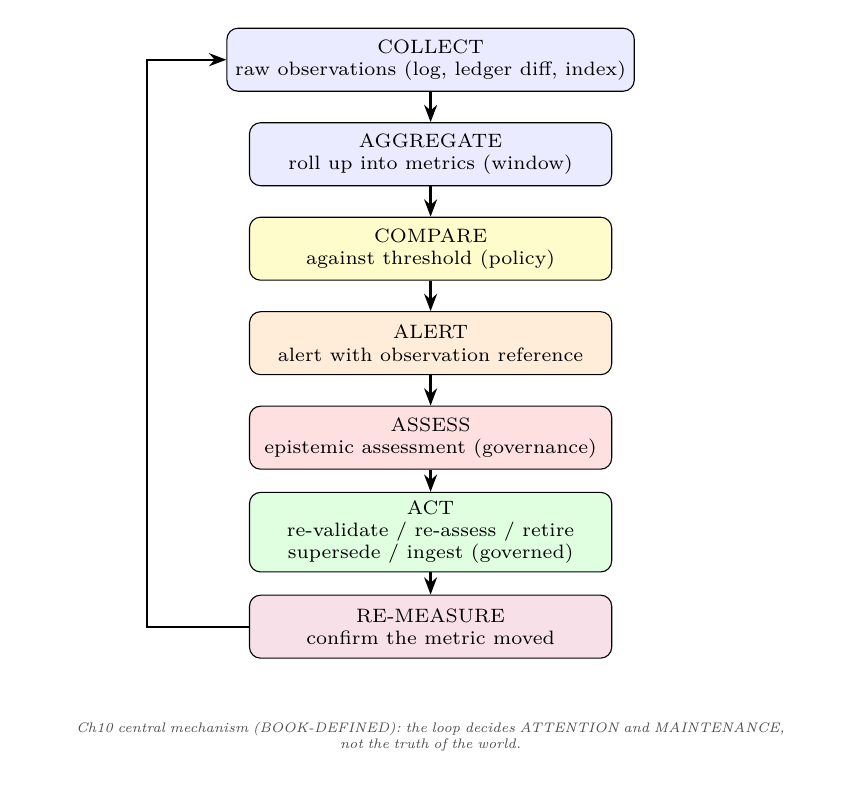
\begin{tikzpicture}[
  box/.style={rectangle, draw, rounded corners, align=center, font=\scriptsize, inner sep=3pt},
  stag/.style={box, minimum width=4.6cm, minimum height=0.8cm},
  arrow/.style={-{Stealth[length=2.2mm]}, thick},
  label/.style={font=\tiny\itshape, text=gray!60!black},
]

% === THE MONITORING LOOP (central mechanism) ===
\node[stag, fill=blue!8]  (collect) at (0, 4.6) {COLLECT\\raw observations (log, ledger diff, index)};
\node[stag, fill=blue!8]  (agg)     at (0, 3.4) {AGGREGATE\\roll up into metrics (window)};
\node[stag, fill=yellow!20](compare) at (0, 2.2) {COMPARE\\against threshold (policy)};
\node[stag, fill=orange!15](alert)   at (0, 1.0) {ALERT\\alert with observation reference};
\node[stag, fill=red!12]  (assess)  at (0,-0.2) {ASSESS\\epistemic assessment (governance)};
\node[stag, fill=green!12](act)     at (0,-1.4) {ACT\\re-validate / re-assess / retire\\supersede / ingest (governed)};
\node[stag, fill=purple!12](remeas) at (0,-2.6) {RE-MEASURE\\confirm the metric moved};

\draw[arrow] (collect) -- (agg);
\draw[arrow] (agg)     -- (compare);
\draw[arrow] (compare) -- (alert);
\draw[arrow] (alert)   -- (assess);
\draw[arrow] (assess)  -- (act);
\draw[arrow] (act)     -- (remeas);
\draw[arrow] (remeas)  -| (-3.6, 4.6) -- (collect);

\node[label, align=center, text width=10cm] at (0, -4.0)
  {Ch10 central mechanism (BOOK-DEFINED): the loop decides ATTENTION and MAINTENANCE,\\not the truth of the world.};
\end{tikzpicture}
\end{document}
